\documentclass[11pt,letterpaper]{article}

% ---------- Typography: serif body, sans headings (institutional memo standard) ----------
\usepackage[margin=0.85in,top=0.5in,bottom=0.5in]{geometry}
\usepackage[T1]{fontenc}
\usepackage{mathpazo}            % Palatino body
\usepackage{helvet}              % Helvetica for headings and labels only
\usepackage{microtype}
\usepackage{xcolor}
\usepackage[colorlinks=true,urlcolor=navy,linkcolor=navy]{hyperref}
\urlstyle{sf}
\usepackage{enumitem}
\usepackage{fancyhdr}
\usepackage{lastpage}
\usepackage{graphicx}

\definecolor{navy}{HTML}{1F3864}
\definecolor{midgray}{HTML}{595959}
\definecolor{hairline}{HTML}{C8C8C8}

\linespread{1.0}
\setlength{\parindent}{0pt}
\setlength{\parskip}{2pt}

% ---------- Footer ----------
\pagestyle{fancy}
\fancyhf{}
\renewcommand{\headrulewidth}{0pt}
\fancyfoot[L]{\sffamily\fontsize{7.5}{9}\selectfont\color{midgray}ENNACIRI \textbar\ PREDICTING U.S. BANK DISTRESS \textbar\ JULY 2026}
\fancyfoot[R]{\sffamily\fontsize{7.5}{9}\selectfont\color{midgray}\thepage\ OF \pageref{LastPage}}

% ---------- Section label ----------
\newcommand{\sectionhead}[1]{%
  \vspace{2pt}%
  {\sffamily\bfseries\fontsize{9.5}{12}\selectfont\color{navy}\MakeUppercase{#1}}\par
  \vspace{-9pt}\textcolor{hairline}{\rule{\textwidth}{0.5pt}}\par\vspace{0pt}}

\newcommand{\answer}[1]{#1\par\vspace{2pt}}

% Quoted block for the LLM text
\newcommand{\quoteblock}[1]{%
  \vspace{1pt}\par
  {\leftskip=20pt \rightskip=20pt \itshape\color{midgray}#1\par}
  \vspace{3pt}}

\begin{document}

% ---------- Title block ----------
\vspace*{-18pt}
{\sffamily\fontsize{8.5}{11}\selectfont\color{midgray}MSDS 696 DATA SCIENCE PRACTICUM II \quad\textbar\quad WEEK 3 INSIGHT REWRITE}\par\vspace{8pt}
{\sffamily\bfseries\fontsize{17}{21}\selectfont\color{navy}Insight Rewrite}\par\vspace{5pt}
{\sffamily\fontsize{9}{12}\selectfont Oussama Ennaciri \quad\textbar\quad Week 3 \quad\textbar\quad July 19, 2026}\par\vspace{4pt}
\textcolor{navy}{\rule{\textwidth}{1.2pt}}

% ---------- The figure ----------
\sectionhead{The figure}
\vspace{2pt}
\begin{center}
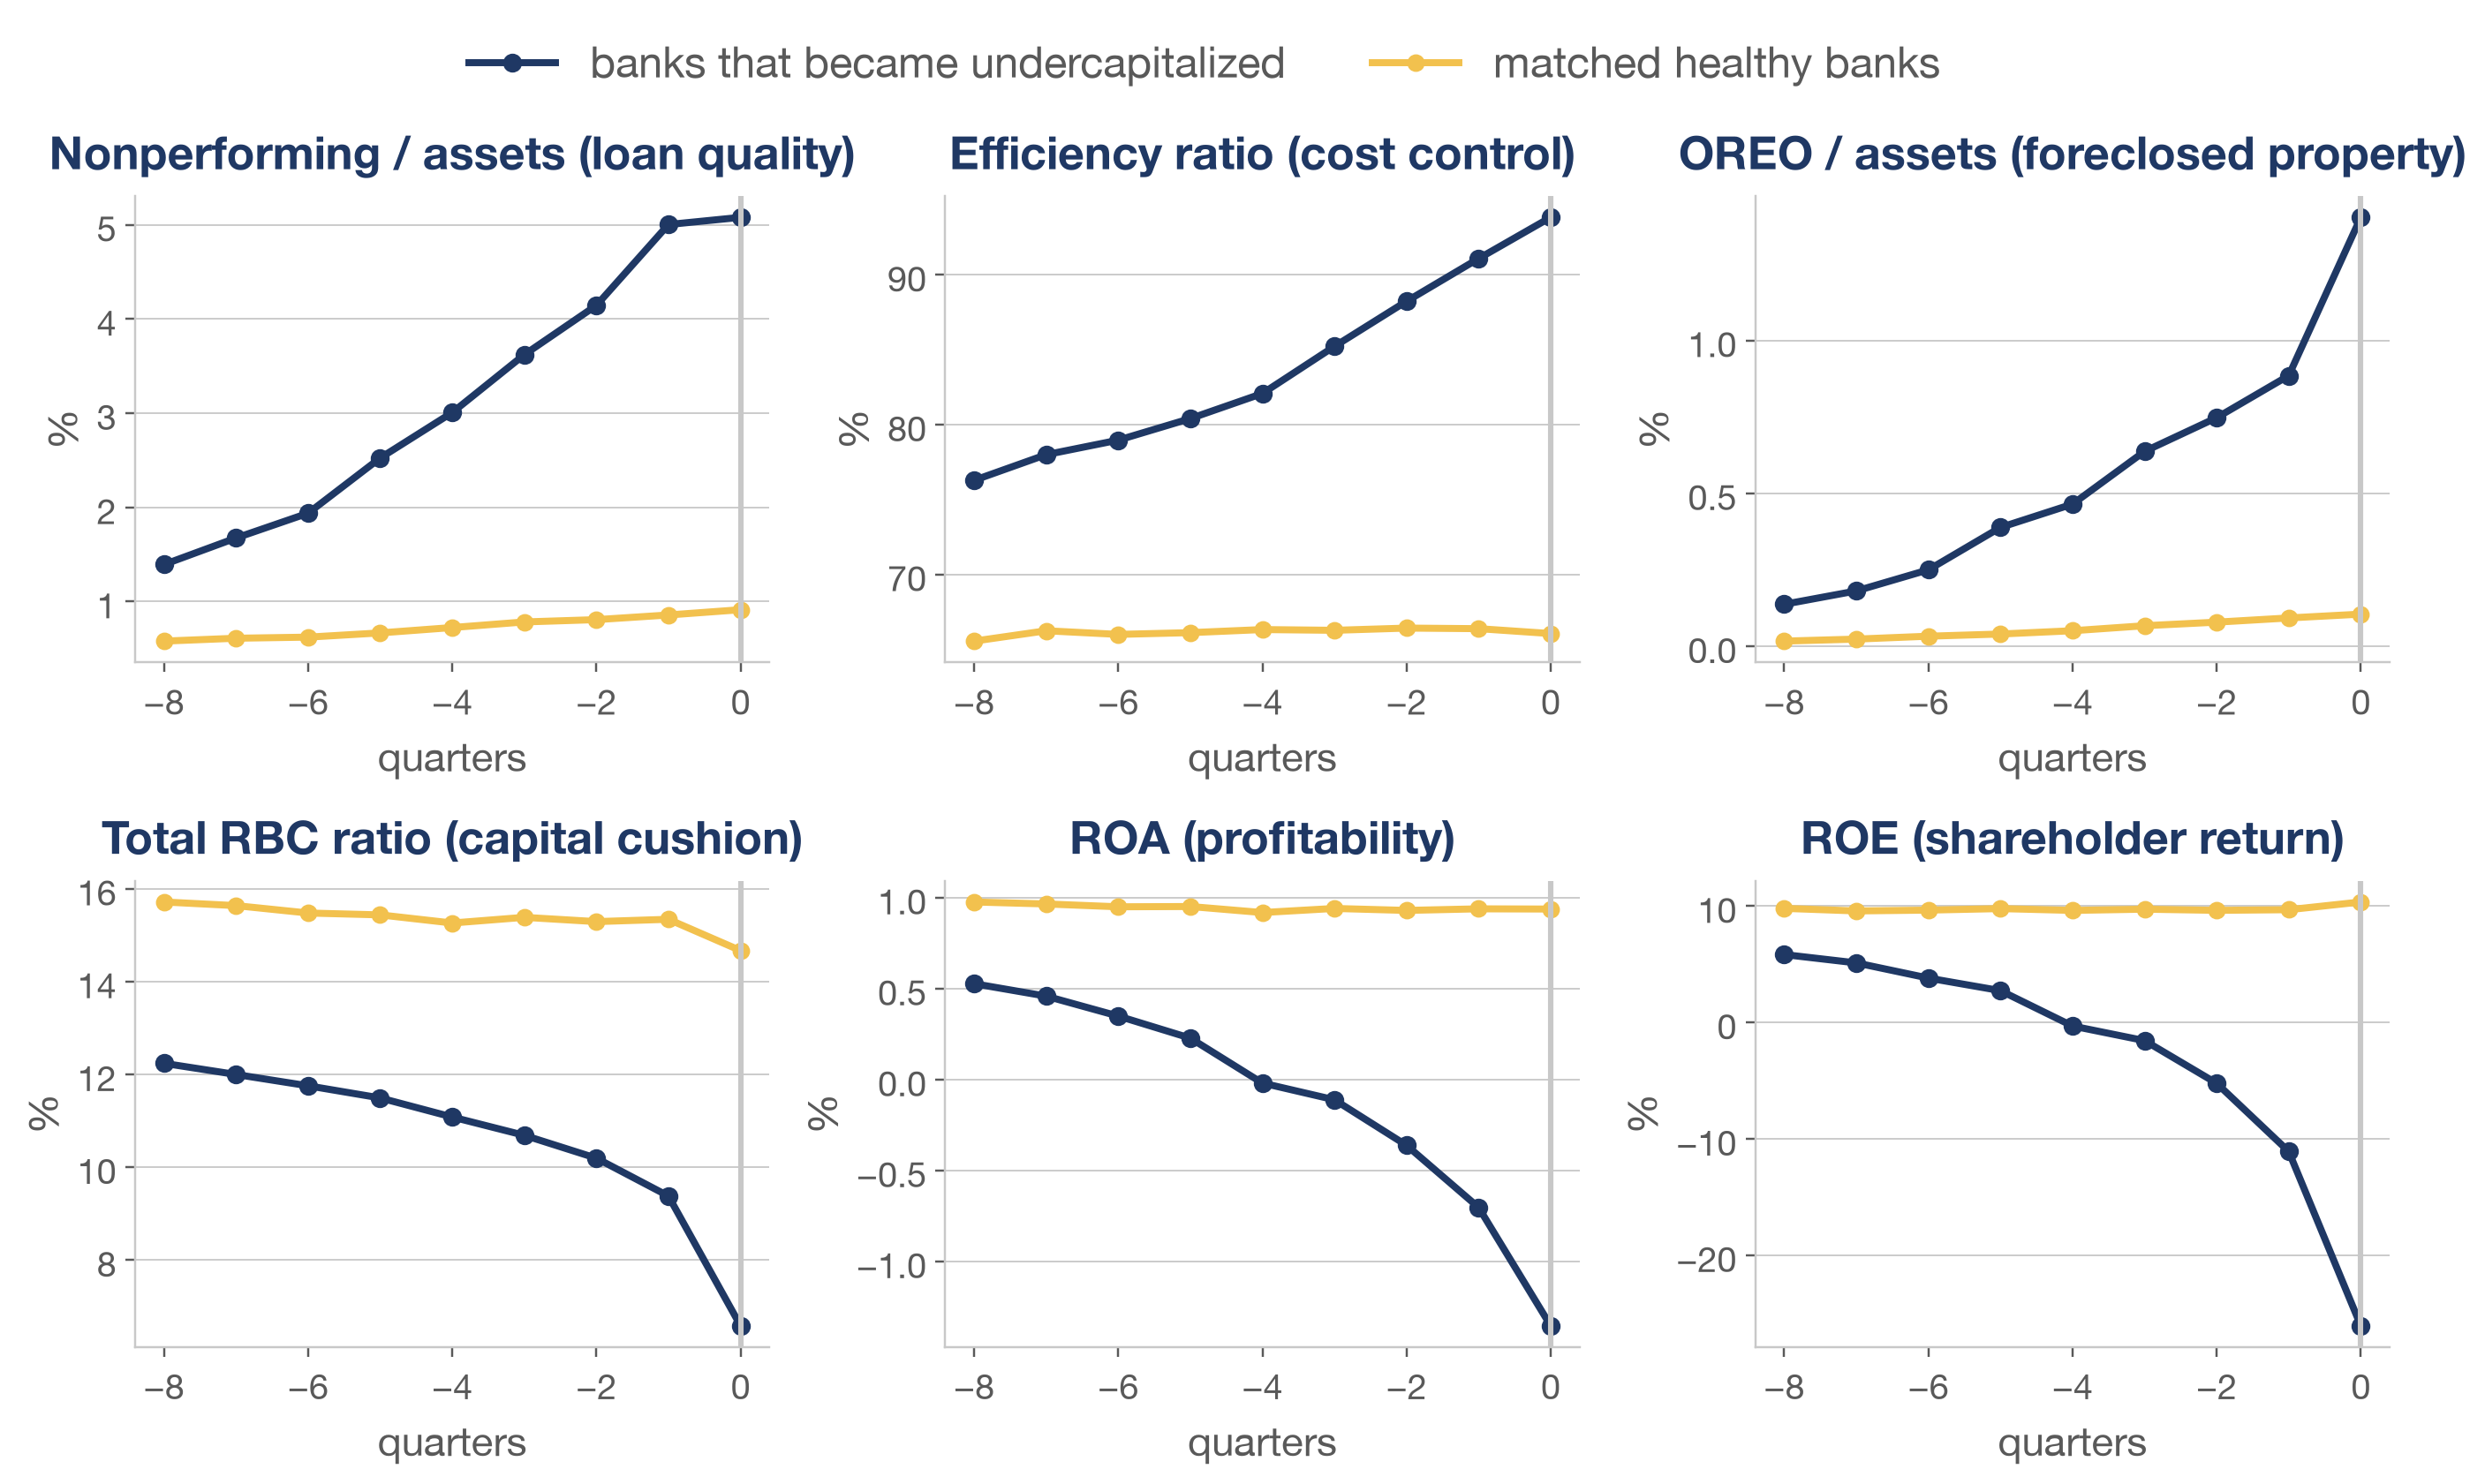
\includegraphics[width=\textwidth]{assets/road_to_trouble.png}
\end{center}

% ---------- The LLM version ----------
\sectionhead{What the LLM wrote}
\answer{I asked an LLM to describe this figure:}

\quoteblock{This chart illustrates the evolution of six key financial metrics in the quarters leading up to a distress event. Nonperforming assets, the efficiency ratio, and other real estate owned trend upward, while capital, ROA, and ROE trend downward. Overall, the figure provides valuable insights into the dynamics of banks approaching distress and highlights the importance of monitoring these indicators.}

% ---------- Why it fails + how I built it ----------
\sectionhead{What's missing}
\answer{The LLM reads the chart back without saying what it means or what to do. It also stopped at the three ratios the literature suggests (capital, nonperforming assets, ROA). I tested every candidate and three more actually move (efficiency ratio, OREO, ROE). I added matched healthy banks to compare against, and analyzed individual distressed banks to make sure the effect is real.}

% ---------- The rewrite ----------
\sectionhead{The rewrite}
\answer{\textbf{Describe.} Banks that end up undercapitalized decline for two years on all six measures; healthy banks stay flat.

\textbf{Interpret.} The decline is bank-specific, not the economy. Signs of distress appear two years before the event, and the decline is mostly gradual, not sudden.

\textbf{Implication.} If I built the model on trends, it is possible to flag a bank before it faces distress.}

% ---------- LLM note ----------
{\small\itshape\color{midgray}\textbf{Note on LLM use:} The quoted paragraph was generated by an LLM at my request, as the assignment asks. This document was typeset in LaTeX using Claude Code. All content, research, and decisions are my own.}

\end{document}
